\subsection{Untersuchung des Linearverstärkers}
Es werden drei Konfigurationen des Linearverstärkers nach Skizze \ref{fig:03} aufgebaut und vermessen. Die Versorgungsspannung beträgt $\left|V_{\pm}\right|=15\si{\volt}$ (symmetrisch). Die verwendeten Widerstände sind in Tabelle \ref{tab:Data_a} aufgelistet und die Messdaten in Abbildung \ref{fig:Plot_a} dargestellt. Mit einer (logarithmischen) Ausgleichsgerade der Form
\begin{equation}
  \text{log}\left(\left|\frac{U_a}{U_e}\right|\right) = a\text{log}\left(\frac{\nu}{\text{Hz}}\right) + b
  \label{eqn:log_fit}
\end{equation}
lassen sich die Parameter aus Tabelle \ref{tab:Fit_a} berechnen. $V_{\text{Plateau}}$ ist hierbei der Mittelwert der Verstärkung im Plateau und $\nu_{\text{Grenz}}$ die Frequenz, bei der die Verstärkung auf $\frac{1}{\sqrt{2}}$ abgefallen ist.
Die Plateaus sind in allen drei Konfigurationen eindeutig zu erkennen, die tatsächliche Verstärkung stimmt aber nicht mit der theoretischen überein. Für die ersten zwei Konfigurationen kann die konvergierende Kurve zu höheren Frequenzen nachgewiesen werden, aber die dritte Konfiguration sticht hierbei ebenfalls heraus.
\FloatBarrier
\begin{table}
  \centering
  \caption{Widerstandswerte und theoretische Verstärkungen in den drei vermessenen Konfigurationen.}
  \label{tab:Data_a}
  \begin{tabular}{c|ccc}
    \toprule
              & $R_1$              & $R_2$               & $V_{\text{ideal}}$\\
    \midrule
    Aufbau 1  & $1\si{\kilo\ohm}$  & $100\si{\kilo\ohm}$ & $100$\\
    Aufbau 2  & $10\si{\kilo\ohm}$ & $150\si{\kilo\ohm}$ & $15$\\
    Aufbau 3  & $100\si{\ohm}$     & $330\si{\ohm}$      & $3.3$\\
    \bottomrule
  \end{tabular}
\end{table}
\FloatBarrier
\FloatBarrier
\begin{table}
  \centering
  \caption{Fitwerte und tatsächliche Verstärkungen in Plateaus, sowie die Grenzfrequenz $\nu_{\text{Grenz}}$ in den drei vermessenen Konfigurationen. In der dritten Konfiguration konnte der Anfang des abfallenden Bereichs nachgewiesen werden, aber nicht genug um einen Fit zu erstellen.}
  \label{tab:Fit_a}
  \begin{tabular}{c|ccccc}
    \toprule
              & $a$              & $b$               & $V_{\text{Plateau}}$ & $\nu_{\text{Grenz}}/\,\text{kHz}$ & VBP $\left(V_{\text{Plateau}}\nu_{\text{Grenz}}\right)/\,\text{kHz}$\\
    \midrule
    Aufbau 1  & $-0.670\pm 0.018$  & $9.75\pm 0.18$ & $34.44$ & $18\pm 7$ & $620\pm 230$\\
    Aufbau 2  & $-0.645\pm 0.012$  & $9.27\pm 0.12$  & $32.4$  & $18\pm 7$ & $440\pm 120$\\
    Aufbau 3  & -         & -       & $37.24$ & -        & -\\
    \bottomrule
  \end{tabular}
\end{table}
\FloatBarrier
\FloatBarrier
\begin{figure}
  \centering
  \includegraphics[width=0.8\textwidth]{build/plot_U_f_a.pdf}
  \caption{Spannungsverstärkung gegen der Frequenz der in Tabelle \ref{tab:Data_a} aufgelisteten Konfigurationen eines Linearverstärkers nach Skizze \ref{fig:03}. Die Plateaus und der Abfall der Spannung bei steigender Frequenz sind gut erkennbar, passt aber nicht mit der Theorie zusammen. Die Ausgleichsgeraden sind über den gefitteten Bereich dargestellt und nach Gleichung \ref{eqn:log_fit} mit den Fitwerten aus der Tabelle \ref{tab:Fit_a}}
  \label{fig:Plot_a}
\end{figure}
\FloatBarrier
\noindent Im nächsten Schritt wird die Phasenverschiebung zwischen Ein- und Ausgang der Verstärkerschaltung untersucht. Hierzu wird der Verlauf der Phasenverschiebung gegen die Frequenz in Abbildung \ref{fig:Plot_b} aufgetragen. Auffälig ist der Vergleich zur Verstärkungskurve aus Abbildung \ref{fig:Plot_a}. Die Phase startet nahe $0$° und steigt in den gleichen Bereichen, wie die Verstärkung abfällt. Die lineare Verstärkung wird hier mit nicht-linearer Verstärkung überlagert und dadurch verringert.
\FloatBarrier
\begin{figure}
  \centering
  \includegraphics[width=0.8\textwidth]{build/plot_phi_f_a.pdf}
  \caption{Phasenverschiebung gegen der Frequenz der in Tabelle \ref{tab:Data_a} aufgelisteten Konfigurationen eines Linearverstärkers nach Skizze \ref{fig:03}.}
  \label{fig:Plot_b}
\end{figure}
\FloatBarrier
\subsection{Untersuchung des Umkehr-Integrator}
Im folgenden wird eine Umkehr-Integrator-Schaltung nach Skizze \ref{fig:04} untersucht. Hierbei ist zu beachten, dass die Ausgangsspannung einem Integral der Eingangsspannung nach der Gleichung
\begin{align}
  U_a &= -\int \frac{U_e(2\pi \nu t)}{RC}\text{d}t\\
      &= -\frac{2\pi\nu}{RC} \int U_e(t') \text{d}t'
\end{align}
folgen sollte. Da in diesem Versuch nur die Maximalspannungen gemessen wurden, kann das offene Integral mittels der Maximumsbeziehung umgeschrieben werden zu
\begin{equation}
  \left|\frac{\text{max}\left(U_a\right)}{\text{max}\left(U_e\right)}\right| \sim \frac{2\pi\nu}{RC}.
\end{equation}
In den Daten sollte eine lineare Beziehnug zwischen Frequenz und Ausgangsspannung ersichtlich werden. Die Daten sind in Abbildung \ref{fig:Plot_c} dargestellt. Offensichtlich herrscht hier keinerlei lineare Beziehung zwischen Ein- und Ausgangsspannung.
\FloatBarrier
\begin{figure}
  \centering
  \includegraphics[width=0.8\textwidth]{build/plot_U_f_c.pdf}
  \caption{Verstärkung eines sinus-förmigen Eingangssignal in einen Integrator aufgebaut nach Skizze \ref{fig:04}. Die erwarte Proportionalität zwischen Verstärkung und Frequenz ist nicht zu beobachten.}
  \label{fig:Plot_c}
\end{figure}
Die integrierenden Eigenschaften des Integrators können mittels der Bilder vom Oszilloskop in den Abbildungen \ref{fig:Osz_c} bestätigt werden.
\FloatBarrier
\FloatBarrier
\begin{figure}
  \centering
  \begin{subfigure}{0.35\textwidth}
    \centering
    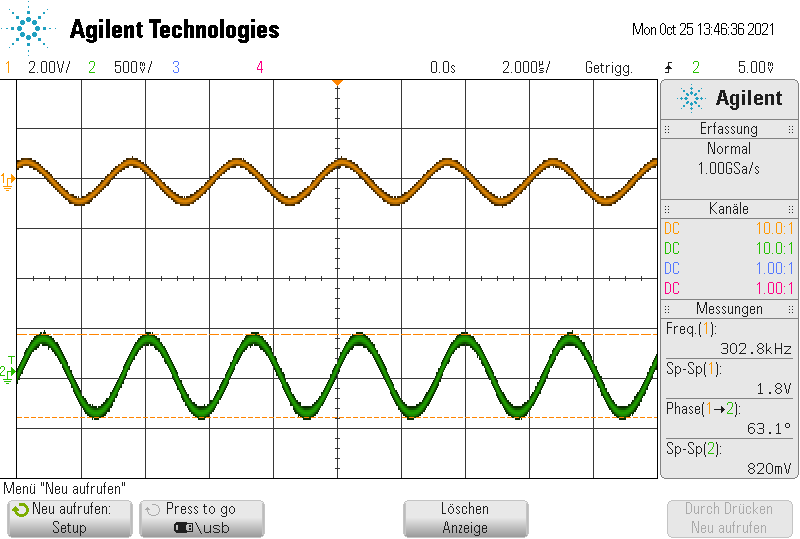
\includegraphics[width=\textwidth]{ressources/integral_sinus.png}
    \subcaption{Integrierte Sinusspannung}
  \end{subfigure}
  \begin{subfigure}{0.35\textwidth}
    \centering
    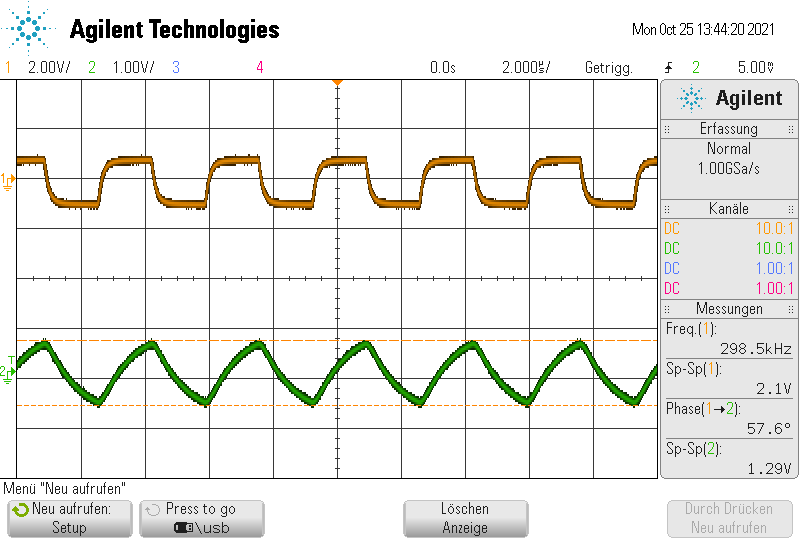
\includegraphics[width=\textwidth]{ressources/integral_rechteck.png}
    \subcaption{Integrierte Rechtecksspannung}
  \end{subfigure}
  \begin{subfigure}{0.35\textwidth}
    \centering
    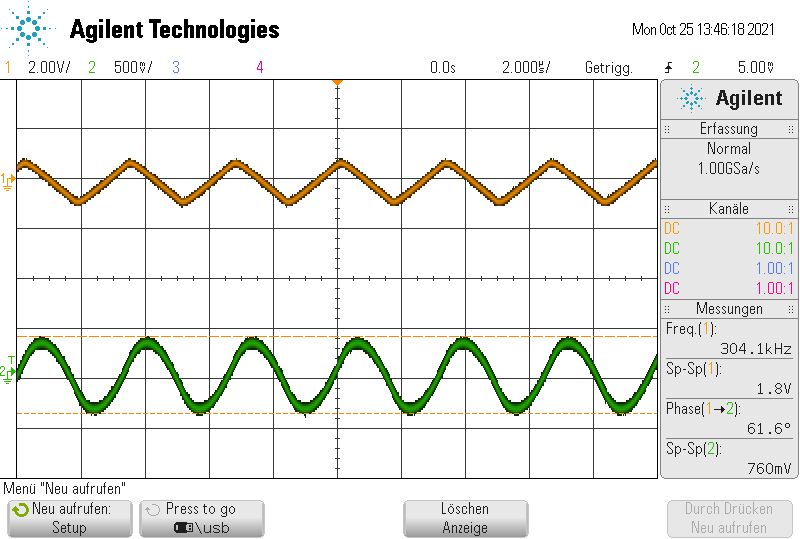
\includegraphics[width=\textwidth]{ressources/integral_dreieck.png}
    \subcaption{Integrierte Dreiecksspannung}
  \end{subfigure}
  \caption{Graphische Aufnahme des Oszilloskops der Ein- (gelb) und Ausgangsspannung (grün) beim Aufbau eines Integrator nach Skizze \ref{fig:04}. Die integrierenden Eigenschaften des Aufbaus sind erkennbar bis gut erkennbar.}
  \label{fig:Osz_c}
\end{figure}
\FloatBarrier
\subsection{Untersuchung des invertierenden Differenzierer}
Im folgenden wird eine Umkehr-Integrator-Schaltung nach Skizze \ref{fig:04} untersucht. Hierbei ist zu beachten, dass die Ausgangsspannung einem Integral der Eingangsspannung nach der Gleichung
\begin{align}
  U_a &= -RC\frac{\text{d}U_e(2\pi \nu t)}{\text{d}t}\\
      &= -\frac{RC}{2\pi\nu} \frac{\text{d}U_e(t')}{\text{d}t'}
\end{align}
folgen sollte. Da in diesem Versuch nur die Maximalspannungen gemessen wurden, kann das Differential mittels der Maximumsbeziehung umgeschrieben werden zu
\begin{equation}
  \left|\frac{\text{max}\left(U_a\right)}{\text{max}\left(U_e\right)}\right| \sim \frac{RC}{2\pi\nu}.
\end{equation}
In den Daten sollte also eine anti-proportional Beziehnug zwischen Frequenz und Ausgangsspannung ersichtlich werden. Die Daten sind in Abbildung \ref{fig:Plot_c} dargestellt. Als Fit wird hier wieder eine lineare Ausgleichsgerade der doppel-logarithmierten Daten
\begin{equation}
  \text{log}\left(\left|\frac{\text{max}\left(U_a\right)}{\text{max}\left(U_e\right)}\right|\right) = a\text{log}\left(\nu \right)+b
\end{equation}
an dem geeigneten Bereich verwendet. Es ergeben sich die Fit-Parameter
\begin{align}
  a &= -0.65\pm 0.04\\
  b &= 9.5\pm 0.4
\end{align}
Wäre die antiproportionale Beziehnug gegeben, wäre $a=-1$. $a$ ist zwar negativ, aber mit geringer Unsicherheit stark von 1 verschieden und damit kann die Antiproportionalität nicht bestätigt werden.
\FloatBarrier
\begin{figure}
  \centering
  \includegraphics[scale=0.8]{build/plot_U_f_d.pdf}
  \caption{Verstärkung eines sinus-förmigen Eingangssignal in einen Differenzierer aufgebaut nach Skizze \ref{fig:05}. Die erwarte Antiproportionalität zwischen Verstärkung und Frequenz ist nicht zu beobachten.}
  \label{fig:Plot_d}
\end{figure}
Die differenzierenden Eigenschaften des Differenzierers können mittels der Bilder vom Oszilloskop in den Abbildungen \ref{fig:Osz_d} nicht klar bestätigt werden.
\FloatBarrier
\FloatBarrier
\begin{figure}
  \centering
  \begin{subfigure}{0.35\textwidth}
    \centering
    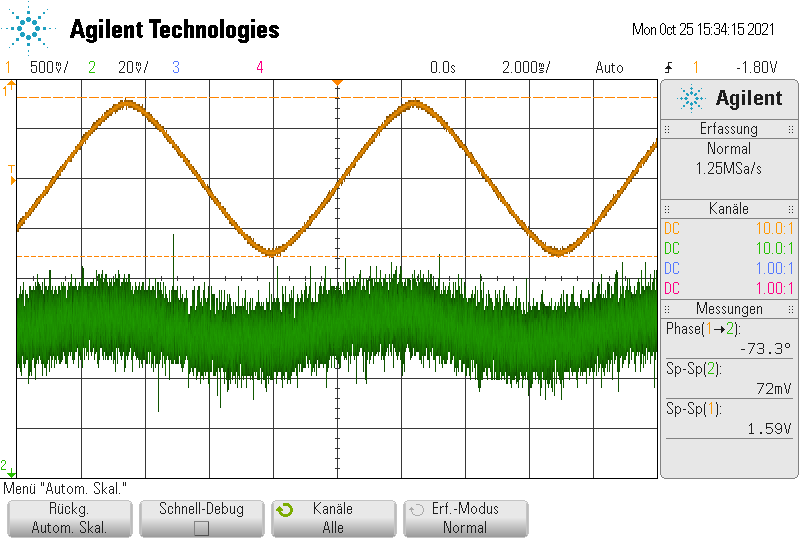
\includegraphics[width=\textwidth]{ressources/differential_sinus.png}
    \subcaption{Differentierte Sinusspannung}
  \end{subfigure}
  \begin{subfigure}{0.35\textwidth}
    \centering
    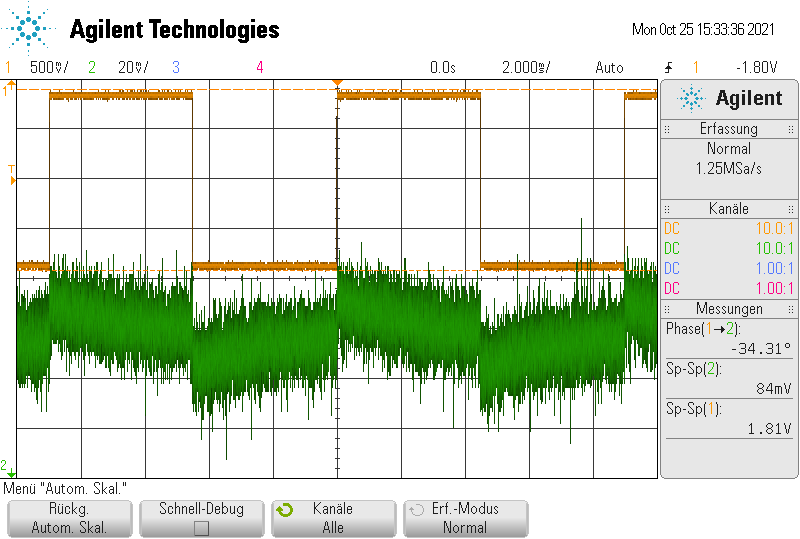
\includegraphics[width=\textwidth]{ressources/differential_rechteck.png}
    \subcaption{Differentierte Rechtecksspannung}
  \end{subfigure}
  \begin{subfigure}{0.35\textwidth}
    \centering
    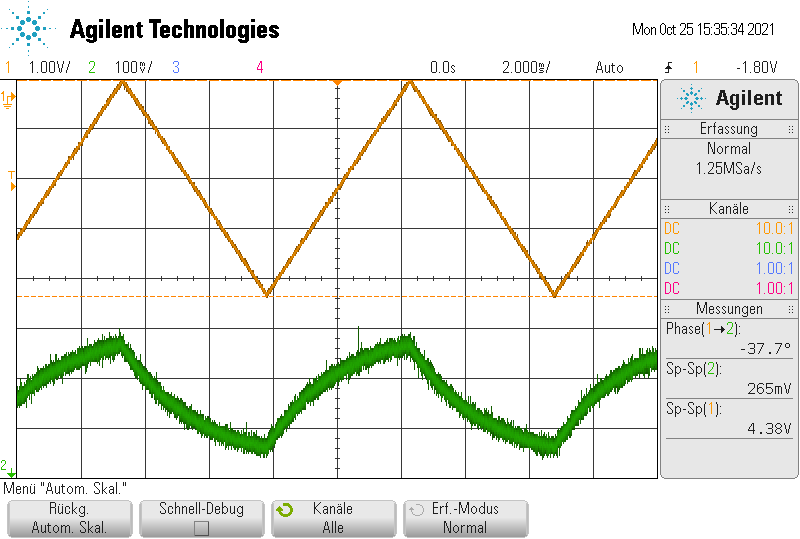
\includegraphics[width=\textwidth]{ressources/differential_dreieck.png}
    \subcaption{Differentierte Dreiecksspannung}
  \end{subfigure}
  \caption{Graphische Aufnahme des Oszilloskops der Ein- (gelb) und Ausgangsspannung (grün) beim Aufbau eines Differenzierers nach Skizze \ref{fig:05}. Die differenzierenden Eigenschaften des Aufbaus sind mit gutem Willen erkennbar, aber zu verrauscht, als das eine definitive Aussage getroffen werden könnte.}
  \label{fig:Osz_d}
\end{figure}
\FloatBarrier
\subsection{Untersuchung des Schmitt-Triggers}
Im folgenden werden die Schwellwerte eines Schmitt-Triggers aufgebaut nach \ref{fig:06} untersucht. Die technischen Daten des Aufbaus sind:
\begin{align}
  U_{A,+} &= 15\si{\volt}\\
  U_{A,-} &= 15\si{\volt}\\
  U_{1}   &= 2\si{\volt}\\
  R_{1}   &= 100\si{\ohm}\\
  R_{2}   &= 220\si{\kilo\ohm}
\end{align}
Mit Gleichung \ref{eqn:09} ergibt sich ein theoretischer Schwellwert von
\begin{equation}
  \left|U_{kipp,\pm}\right| = 6.82\si{\milli\volt}
\end{equation}
und die gemessenen Schwellwerte liegen bei
\begin{align}
  U_+ &= 87 \si{\milli\volt}\\
  U_- &= -230 \si{\milli\volt}.
\end{align}
Mit Abweichungen von mehr als einer Zehnerpotenz kann damit die Theorie nicht bestätigt werden.
